

\chapter{Background}
\label{chapter:background}

\begin{introduction}
    
    The modelling of the energy consumption of the \ac{ict} sector is a complex task, because it involves modelling several systems, each with their distinct topologies and external factors.

    In this chapter we can find a description of the topology of the different systems that comprise the \ac{ict} sector and a highlight on the main component of each system. Moreover, the chapter also includes a description on the basics of compression algorithms and the different types of compression algorithms.

\end{introduction}

\section{System Boundaries}
\label{section:system_boundaries}

The definition of system boundaries is an important factor in the modelling of energy consumption. As seen in the compilation of studies made by \citet{Aslan2018}, the system boundaries are one of the main factors for the discrepancies of the results.

The common consensus is that the system boundaries for the model of the internet should exclude datacenters and user devices \citet{Coroama2014}. This study however won't be modeling only the internet but also the impact on datacenters and of the compression/decompression algorithm in the end user device. So the overall system boundary will include all the \ac{ict} sector. 

So this study divides the system boundary in 3 main components, the network, datacenters and the end user devices (figure \ref{figure:system_boundaries}). The network is divided in three main components, \ac{cpe}, Access Network and Core Network. The datacenter is also divided in three components, Servers, Storage and Datacenter Network. Lastly the end user devices only includes the compression/decompression algorithm cost. 

\section{Internet}

The internet is the most complex component of the model.
Internet started has an interconnection of small number of local university networks, which were composed of a few routers and cables. Nowadays, the internet is a global network of networks, composed of millions of routers, switches and cables, that interconnects billions of end users. This communication is made possible by the use of the \ac{tcp} and \ac{ip} protocols.

Because of its complexity the system is usually divided in smaller components, however the delimitation on where each component begins and ends can vary from paper to paper. In this thesis we use the delimitation proposed by \citet{Coroama2015} and \citet{Schien2015}, which divides the internet in 4 main components: \ac{cpe}, access network, \ac{ip} core network and undersea cables.

\ref{fig:internet_topology} shows the topology of the internet as described by both papers \cite{Coroama2015} \cite{Schien2015}. 

\subsection{\acl{cpe} and Access Network}

There are several technologies used to establish to connect user to the Ethernet, they can be either wired or wireless and can be part of the \ac{cpe} layer or access network layer. Figure \ref{figure:network_technologies} highlights which technologies are currently used and in what layer they belong to.

\begin{figure}[h]
    \centering
    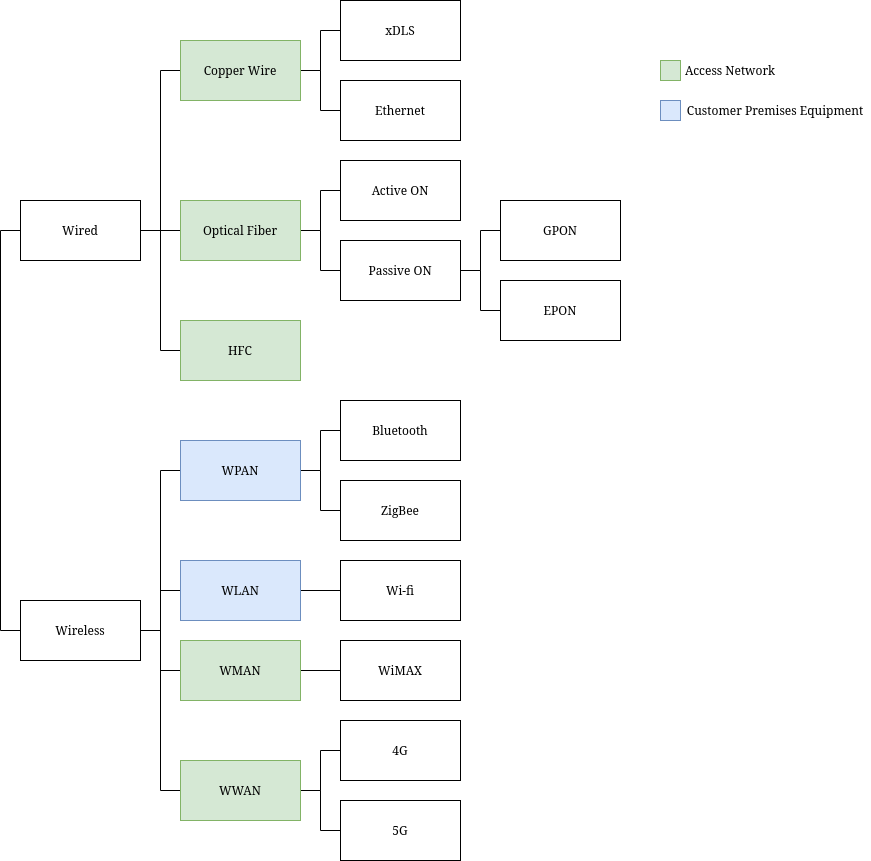
\includegraphics[width=0.8\textwidth]{figs/network_technologies.png}
    \caption[Network technologies used in Access Networks and CPE]{Network technologies used in Access Networks and CPE. In green are the technologies used in the access network and in blue are the technologies used in the CPE. Adapted from \citet{forum:huwawei}}
    \label{figure:network_technologies}
\end{figure}

The first layer and most simple is the \ac{cpe}. The \ac{cpe} is the equipment that is installed in the end user premises. 
The equipment is usually provided by the \ac{isp} and normally consists of a gateway that acts as a modem and a router.
A modem is used to convert the signal from the \ac{isp} to a signal that can be used by the router. The router is used to connect the end user devices to the internet. The user can connect to the routers either by cable or by wireless technology like Wi-fi. 

Access networks serve as the connection between the \ac{cpe} and the core network. All the user are connected to a central office where traffic is aggregated and then transferred to the core network.
The access network incorporates any technology that establishes the connection between the end user and the \ac{isp} and said technology it is not own by the user. % So a user can connect to the internet by either a modem or a cellular tower but only the cellular tower is part of the access network. 

Traffic in the access network is highly variable. The equipment used in the access network has a power consumption that is largely constant in time and thus load-independent \citet{Heddeghem2011}.

\subsubsection{Access Network Wired technologies}

The most popular wired connections are \ac{dsl}, coax cable and fiber-optics.

\begin{itemize}

    \item \ac{dsl} provide internet access over existing analog telephone lines. So, existing telephone service providers offer \ac{dsl} service. With this technology, user voice and data traffic go through this analog lines. \ac{dsl} uses high frequencies for data transmission. And with a help of \ac{dsl} filter data traffic do not interference with voice traffic.
    There are different DSL types. Now \ac{adsl} is the most used \ac{dsl} type in the world. 

    \item \ac{hfc} uses the same coaxial cable that is used for cable television. It uses the \ac{docsis} standard to provide internet access.

    \item Fiber-optic networks use light pulses transmitted through glass or plastic fibers, which produce high bandwidth and transmit speeds. 
    The fibers are also more resistant to interference and signal degradation, making them better suited for sending data over long distances without losing signal quality.
    Fiber optics technology, namely \ac{epon}, have become the most popular choice for wired access network technology. \ac{epon} is a point-to-multipoint network, which means that a single optical fiber is used to serve multiple end users. This is done by using a passive optical splitter, which splits the signal into multiple data streams that are sent to each end user.

\end{itemize}


\subsubsection{Access Network Wireless technologies}

Wireless access networks use radio waves to provide fixed or mobile access services for users. 
According to coverage range classification, the broadband wireless access technology are generally divided into different categories such as \ac{wpan}, a \ac{wlan}, a \ac{wman}, and a \ac{wwan}, however only technologies in the \ac{wman} and \ac{wwan} fall into the umbrella of what we refer as the access network.

The area coverage of \ac{wman} is in the order of kilometers and there are 2 prominent technologies for establish internet access, \ac{lmds} and \ac{wimax}.

\begin{itemize}

    \item \ac{lmds} as the name says is a multipoint communication system, it is used to provided network connectivity to buildings. These are great technologies for last mile connectivity, because they are more cost-effective than wired technologies and can be deployed faster than fiber \cite{forum:imda}.

    \item \ac{wimax}  is based on IEEE 802.16. It provides fixed, mobile or portable wireless connections with high speeds that can reach up to 70 \ac{mbps} \cite{forum:ctrfantennasinc}.

\end{itemize}

The \ac{wwan} has a bigger range that the \ac{wman} and is used to provide internet access to mobile devices.
\ac{wwan} uses telecommunication cellular network technologies such as 2G, 3G, 4G LTE, and 5G to transfer data.


\subsection{Core Network}

Core networks consist of several core nodes that are interconnected by \ac{wdm} optical fiber links.

\ac{wdm} is a fiber-optic transmission technique that enables the use of multiple light wavelengths (or colors) to send data over the same medium. Two or more colors of light can travel on one fiber, and several signals can be transmitted in an optical waveguide at differing wavelengths or frequencies on the optical spectrum. 

Each core node is composed by a mix of several layers of technologies stacked on top of each other. Typically, it is composed of a \ac{ip} layer, a \ac{wdm} layer and a \ac{oxc} layer.

From a broad perspective, core nodes operate on an optical-electrical-optical basis. This implies that any optical traffic undergoes conversion into the electronic domain and is then processed by the node, regardless of whether the traffic is terminated at that node. Typically, a node comprises several \ac{wdm} transmit and receive cards, commonly known as transponders or transceivers, which are linked to an \ac{ip} router. The \ac{ip} router, in turn, can establish connections with various access routers.

\section{Datacenters}

Datacenters are facilities that house numerous computing and storage devices. They provide users with the opportunity to host their applications as well as store data. Their use is widespread, and their energy impact is substantial, as they are responsible for X\% of the global energy consumption \cite{get source}.

Datacenters are composed of electronic equipment for communication, data processing and storage. The quantity and type of equipment depends on the type of datacenter. Usually you can distinguish the type of datacenter by its size and processing power. \citet{US-report2016} classifies datacenters in the following categories:

\begin{itemize}
    \item Closet
    \item Room
    \item Localized
    \item Midtier
    \item High-end
    \item Hyperscale
\end{itemize}

The main contributors for the energy consumption of datacenters are the servers, the network and the storage devices. Each type of datacenter has a different efficiency in the use of energy. The efficiency of a datacenter is measured by the \ac{pue}, it is the ratio between the total energy consumption of the facility and the energy consumption of the \ac{it} equipment, the closer it is to 1 the better the efficiency of the datacenter.

\subsection{Datacenter Servers}

Datacenter servers are the main component of the datacenter. The servers are computers with the resources capable of executing applications and processing data.

As the main component of the datacenter, they are also the main contributor for the energy consumption of it. According to \citet{Cheung} and \citet{Miyuru} the servers account for around 70\% of the energy consumption of the datacenter, ignoring cooling and other non \ac{it} factors.


\subsection{Datacenter Storage}

Storage in datacenter is composed of several \acp{hdd} and \acp{ssd} that are connected to the servers. The storage configuration can be divided in three categories: \ac{das}, \ac{nas} and \ac{san} \citet{Storage101}.

\subsubsection{\acl{das}}

As the name suggests, the storage devices connect directly to the server without any networking. \ac{das} can connect either internally or externally has a single drive or an array of \ac{raid}. 

\ac{das} is the cheapest easier and cheapest option to implement of the three. However, it is also the least scalable and the least flexible, because the server has a limited number of ports and expansion slots.

\subsubsection{\acl{nas}}

\ac{nas} is a centralized file-level storage system, that is connected to the server via the network. \ac{nas} is composed of a storage device with a \ac{os} that is optimized for file storage and sharing.

It includes built-in fault tolerance, management capabilities, and security protections, and it can support features such as replication and data deduplication.

\subsubsection{\acl{san}}

\ac{san} is a decentralized block-level storage system, that is connected to the server via the network. It presents a pool of block-level storage to the server, which the server can then format and partition as it sees fit.

It is composed of storage arrays (\acp{raid}), servers for managing data access, storage management software, \acp{hba}, and any physical components that make up the network's infrastructure.

\subsection{Datacenter Network}

Typically, datacenter networks are composed of switches, routers and other hardware components that provide the connectivity and security to run applications and process data on the servers. 
According to \citet{Cheung} and \citet{Miyuru} the network accounts for around 10\% of the energy consumption of the datacenter. 

Today there are 3 main topologies that datacenters can follow, but larger datacenters can use two or all three of them. Each topology has its own advantages and disadvantages and the choice of topology depends on the type of datacenter and the type of applications that it will be hosted \citet{commScope}.

\subsubsection{Centralized}

This model is more used by smaller datacenters. There are separated environments for the server and storage, with dedicated  cables that connect the storage server cabinets to the storage.  

\subsubsection{\ac{eor}}

This topology consists in distributing network resources, as seen in figure \ref{figure:eor_topology}. The servers are placed in rows and the network resources are placed at the end of each row. This solution is recommended by the  ANSI/TIA-942 Data Center Standards \cite{ANSI/TIA-942} and is very scalable, repeatable, and predictable.

\subsubsection{\ac{tor}}

Top of the rack consists on two or more swtches on top of each server cabinate, as shown below in figure \ref{figure:tor_topology}. It is cost-effective because it reduces the number of copper cables between racks. The rack is linked to the data center network by an Ethernet switch, often through a fiber cable. This fiber cable is a direct link from the common aggregation area to the rack.
In the \ac{tor} approach, every rack in the data center network is a separate entity that eases its management. Any change, upgrade, or malfunction in the rack usually affects that rack only.

\section{Compression algorithms}

Compression algorithms are used to reduce the size of a file or data stream. They have been used in applications where the cost of storage or transmission is high.

With the increase of the use of the internet and the increase of the amount of data that is stored and transmitted, compression algorithms have become a standard in the \ac{ict} sector.

\subsubsection{Lossless compression}

Lossless algorithms usually exploit the redundancy present in data to reduce the size without losing any information. Among the lossless algorithms, the Lemple-Ziv (LZ) family of algorithms are the most popular. One popular image format that uses lossless compression is the \ac{png} format. The \ac{png} format uses the DEFLATE algorithm \cite{rfc1951}, which is a combination of LZ77 and Huffman coding.

\subsubsection{Lossy compression}

Lossy compression algorithms are used when the loss of information is acceptable. They are usually used in multimedia applications, where the loss of information is not noticeable by the end user.

Compression algorithms can be divided in two categories based on the type of data that they are used to compressing. General purpose algorithms can be used to compress any type of data. Specific algorithms on the other hand are developed to compress a specific type of data, like images, audio or even genetic data, and are usually more efficient in their data type than general purpose algorithms.

Below we will enumerate some of the most popular compression algorithms, focusing on algorithms that are commonly used to compress genome sequences. But first we will explain the common formats used to store genome sequences.

\subsection{Genome sequence formats}

Genome sequencing is a process that determines the order of the nucleotides in a genome, it turns sequences of genomes into data that can be stored and analyzed. The genome sequence is usually stored in a file, which can be in several formats. The most common formats are FASTQ, FASTA, \ac{sam}/\ac{bam} and \ac{vcf}.

FASTQ is a text-based format that stores the biological sequence and its corresponding quality scores. Each entry of the file is composed of 4 lines. The first line is the sequence identifier, the second line is the genetic sequence (the nucleotide bases A, C, T, G and N), the third line is a separator, lastly the fourth line is the quality score of each base.

FASTA is also a text-based format that stores the biological sequence. However, it only stores the headers and nucleotide bases sequenced, which makes it more compact than FASTQ.

\ac{sam}/\ac{bam} are the text and binary versions of the same format. They are used to store the alignment of the sequenced reads to a reference genome. The file is composed of a header and a body. The header contains information about the reference genome and the body contains the alignment of the reads. They reduce the space needed to store a genetic sequence however they are dependent on a reference genome.

Lastly \ac{vcf} is the standard file format for storing variation data. It is used by large scale variant mapping projects such as IGSR. It is also the standard output of variant calling software such as GATK and the standard input for variant analysis tools such as the VEP or for variation archives like EVA.
VCF is a preferred format because it is unambiguous, scalable and flexible, allowing extra information to be added to the info field. Many millions of variants can be stored in a single VCF file. 

\subsection{Compression algorithms overview}

\subsubsection{General purpose algorithms}

As stated above, compression algorithms can be divided into two categories, general purpose and specific algorithms. In terms of general purpose algorithms, we have the most popular algorithms, zstandard, gzip, bzip2 and lzma.

Zstandard and Gzip are both lossless compression algorithms based on the DEFLATE algorithm, which uses a combination of both LZ77 and Huffman coding. Zstandard is the most recent algorithm and was developed by Facebook, offering a much faster compression and decompression than its predecessors. Gzip was created as an alternative to the compress program in Unix systems, because of the Unisys and IBM patens covering the LZW algorithm.

Bzip2 is a lossless compression algorithm based on the Burrows-Wheeler transform. It is more efficient than DEFLATE but is also slower. Even though it can be used in any type of data it is most efficient in text based data. The algorithm is composed of several compression techniques such as \ac{rle}, Burrows-Wheeler transform, move-to-front transform and Huffman coding.

Lzma is a lossless compression algorithm based on the Lempel-Ziv-Markov chain algorithm. It is used by the 7zip file archiver and the xz file format.

Cmix and paq are both context mixing compression algorithms. They use more than one model to predict the next symbol in a sequence, it usually results in a more accurate prediction than using only one model. Cmix uses several machine learning models, while paq1, a version of the paq, uses a weighted average of 5 bit-level predictors.

Nncp also uses machine learning models, in this case it uses pure neural network models based on the \ac{lstm} and Transform model.

\subsubsection{Specific algorithms}

In terms of specific algorithms, we focus on algorithms that compress genome sequences. These algorithms compress files that are in the FASTA, FASTQ and \ac{sam}/\ac{bam} formats.





\begin{center}
    \begin{tabular}{|| c | c | c | c | c ||}
        \hline
        Name & Data type & Compression Rate & Decompression Speed & Reference \\
        \hline\hline
        1 & 2 & 3 & 4 & 5\\
        \hline
    \end{tabular}
\end{center}


% estado da arte de algoritmos especificos
% algoritmos usados pelo ENA european nucleotide archive e SRA
% zstandard gzip bzip2 lzma 
% especificos fqzcomp quip leon 
% dsrc2 

% tipos de dados:
% fastq fasta sum/bam vcf

% seqSqueeze

% mfcompress
% jarvis3
% naf agc

% cmix
% paq1-9
% nncp



